\subsection{$d(K^-, n)$ scaling factor}
$d(K^-, n)"X"$ spectrum can be converted from counts to the differential cross section ($\frac{d^2\sigma}{d\Omega dm}$) excepting the acceptance of the the CDS that is depend on the reaction.
The parameters was used for the conversion were summarized in Table\ref{tab:KN_scale}.

First one is luminosity which was consist of number of target, number of irradiated kaon, DAQ live rate, trigger efficeincy.
The number of target was defined from length of fiducial volume ($10cm$) and target density which was evaluated from measured tempature.
The number of irradiated kaon was defined by correcting kaon number counted up by the scaler DAQ by ratio of true kaon in kaon trigger which was described in Sec\ref{sec:beam_line_ana}.
About DAQ live rate and trigger efficiency were discribed in Sec\ref{sec:trigger}.
The luminosity was evaluated run-by-run.
In the table, these items were represented value weighted by data statistics as typical value.

Next is about the CDS which was CDC efficiency discribed in Sec\ref{sec:CDC_eff}.
Accpectances of CDS were estimated and corrected by the Monte Carlo simulation data.
These evaluations were described in individual section for each reactions.

Last one is about the NC which was consists of acceptance and efficiency.
The efficiency of the NC was further decomposed to intrinsic one and overveto by the CVC and the BVC that was described in Sec\ref{sec:NC_eff}.
The acceptance of the NC was estimated from the NC position and the error was evaluated from difference of the first layer and the last layer of the NC.

\input{analysis/KN_scaling_table}


\begin{table}
  \caption{
    Summary table of $d(K^-, p)$ scaling parameters
  }

  \hspace{-2cm}
  \begin{tabular}{cc|cc|cc}
    \multicolumn{2}{c|}{Component}  & value            & error           & value  & error \\
    \hline
    \hline
    Luminosity   ($/\mu b$)    &    & 2478             & 81          &  & \\
    & Target Length (cm)       &  & & 10               &                  \\
    & Target density $[g/cm^3]$&  & & 0.1624           & 0.0014           \\
    & Number of Kaon           &  & & 2.05$\times 10^{10}$ &              \\
    & Survival ratio of $K^-$  &  & & 0.336            & 0.0001           \\
    & DAQ live ratio           &  & & 0.821            & 0.0001           \\
    \multicolumn{2}{c|}{Trigger efficiency}  &  & &                  &    \\
    \hline
    & $K \otimes$CDH1          &  & & 0.9527           & 0.0003 \\
    & Charge                   &  & & 0.9559           & 0.0004 \\
    \hline
    \hline
    Efficiency of the CDC      &    & 0.977            & 0.04    &  & \\
    \hline
    %% \hline
    %% Acceptance of the PC/CVC (msr) & & \multicolumn{4}{|c}{Evaluate by the SIM} \\
    \hline
    Efficeincy of the forward detectors  &    & 0.819            & 0.042   &  & \\
    Efficeincy of the FDC1               &    & 0.987            & 0.005   &  & \\
  \end{tabular}
  \label{table:KP_scaling}
\end{table}


The $d(K^-, n)\pi^{\mp}\Sigma^{\pm}$ spectra obtained in the previous subsection and
the $d(K^-, p)\pi^- \Sigma^0$ spectrum obtained in Section \ref{sec:K0_ana}
are scaled by the luminosity, the detection efficiency of detectors, and the solid angle of the forward detector.
Their values are summarized in Table \ref{table:KN_scaling} for $d(K^-, n)\pi^{\mp} \Sigma^{\pm}$
and in Table \ref{table:KP_scaling} for $d(K^-, p)\pi^- \Sigma^0$.
In addition, the acceptance of the CDS, depending on the $\pi \Sigma$ masses,
is evaluated using Monte Carlo simulations generated according to a uniform $\pi \Sigma$ mass distribution,
where $\pi^{\mp} \Sigma^{\pm}$ is as described in the previous section, and $\pi^- \Sigma^0$ is generated in a similar way.

The luminosity consists of the thickness of the target and the number of beams irradiated.
Target thickness is explained in Section \ref{sec:target}.
The number of irradiated beams is divided into the total number of Kaon beams irradiated,
the fraction of these that actually pass through the fiducial volume of the target,
the DAQ live ratio, which is the fraction that the DAQ accumulates as events that can be analyzed,
and the trigger efficiency, which is the fraction of trigger signals produced.
The fraction of beams that pass through the fiducial volume is explained in Section \ref{sec:beam_ana}.
The DAQ live ratio and the trigger efficiency are explained in Section \ref{sec:trigger}.
These values are evaluated for each run and summed up.
The values in the table are representative, and the error represents the fluctuation between runs.

Next is the detection efficiency.
In the case of forward neutrons, $d(K^-, n)\pi^{\mp}\Sigma^{\pm}$, 
the detection efficiencies of the NC for forward neutrons and the CDC for the two charged $\pi$ are taken into account.
The detection efficiency of the CDC is explained in Section \ref{sec:CDC_eff}.
The detection efficiency of the NC is divided into the intrinsic detection efficiency of the NC, as discussed in Section \ref{sec:NC_eff},
and the effect of overkill caused by the CVC and the PC installed to veto charged particles, which is explained in Section \ref{sec:NC_overkill}.
In the case of forward protons, $d(K^-, p)\pi^- \Sigma^0$, the charged $\pi$ were also detected using the CDC,
while the FDC1 and the PC/CVC were used for detecting forward protons.
The detection efficiencies for these detectors are described in Section \ref{sec:FC_eff}.

Next is the solid angle of the forward detector.
In the case of forward neutrons, since the neutron flight path is a straight line, it can be simply calculated from the position of the NC.
The solid angle is estimated from the center position of the NC, and its error is determined by the thickness of the NC.
On the other hand, for forward protons,
the calculation is not straightforward due to the momentum dependence caused by bending from the Beam Sweeping Magnet,
so we used Monte Carlo simulation to evaluate the solid angle.
In that simulation, the effect of multiple scattering was estimated, and other reactions,
such as elastic scattering,inelastic scattering, and hadron reactions, were cut off.
Using that simulation, the forward protons passing through all six planes of FDC1 and the PC/CVC were treated as effective events.
The effective rate was calculated for each infinitesimal piece of solid angle, weighted accordingly,
and then summed together to obtain the total solid angle.
The relationship between the $\pi^- \Sigma^0$ mass and solid angle obtained by this method is shown in Figure \ref{fig:PCCVC_SA}.
%% TODO 絵の更新、合わせたコメント

\begin{figure}[htbp]
  \centering
  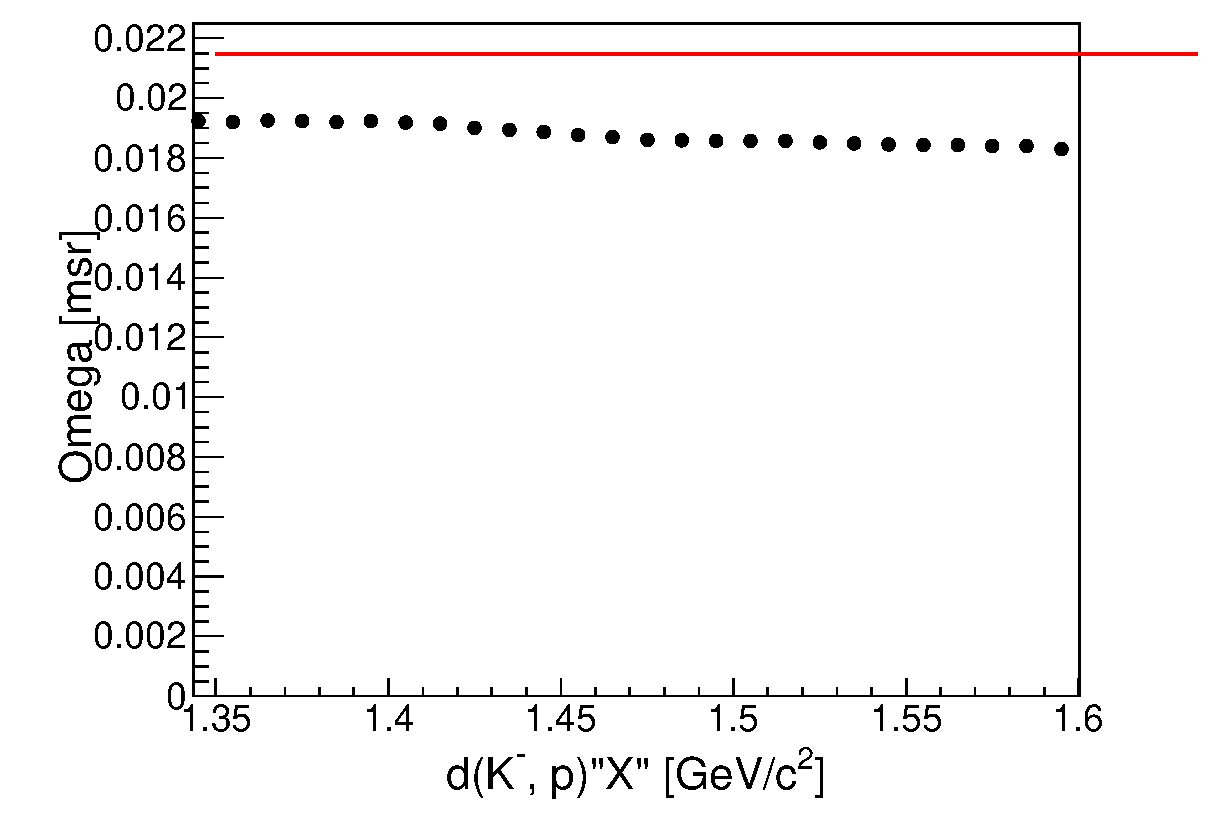
\includegraphics[width=8cm]{../pic/Dron/PCCVC_SA.eps}
  \caption{
    This figure shows the relationship between the mass of the $\pi^-\Sigma^0$ system and
    the solid angles of the forward detectors (FDC1 and PC/CVC) with respect to the outgoing forward proton.
    The red line indicates the solid angle of the NC detector with respect to the forward neutron.
  }
  \label{fig:PCCVC_SA}
\end{figure}


\begin{figure}[htbp]
  \centering
  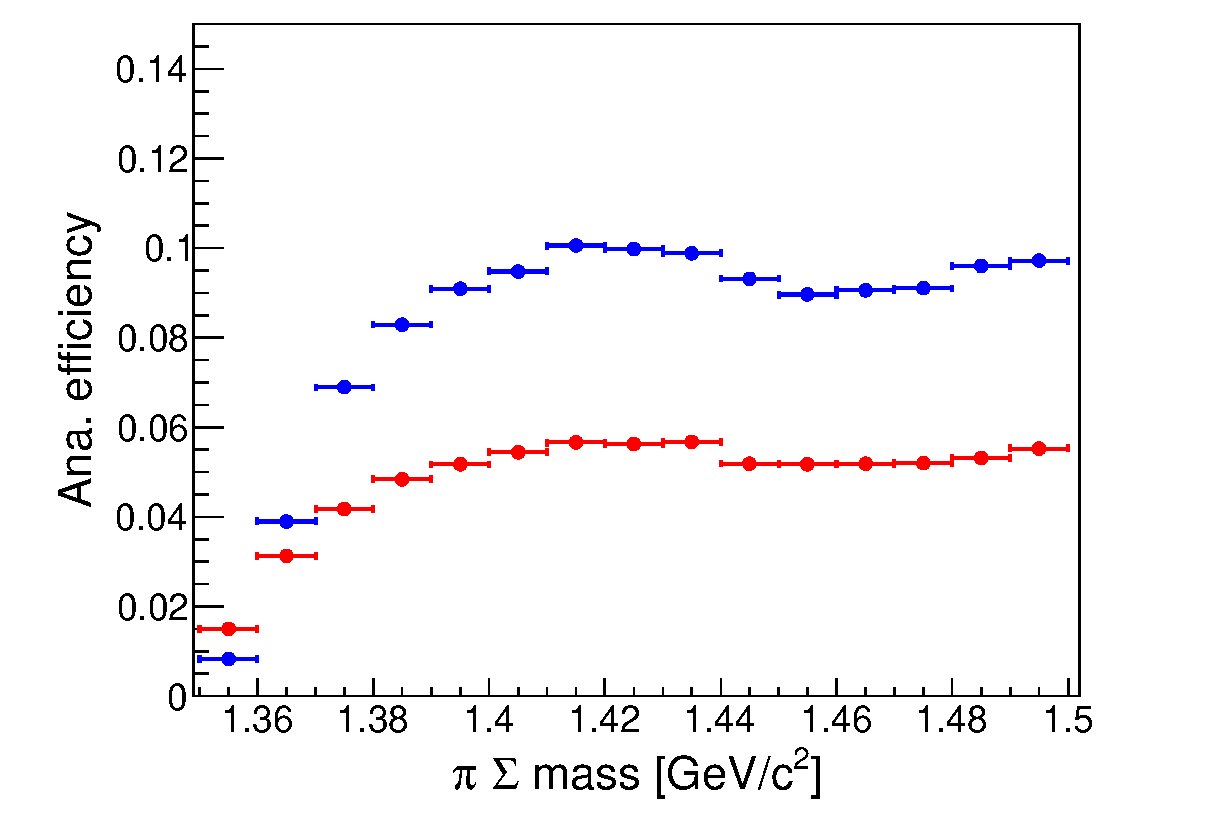
\includegraphics[width=8cm]{../pic/Dron/KN_ana/kn_acc.eps}
  \caption{
    This figure shows the acceptance of $d(K^-, n)"\pi^{\mp}\Sigma^{\pm}"$.
    The red line indicates $\pi^- \Sigma^+$ and the blue line indicates $\pi^+ \Sigma^-$.
  }
  \label{fig:kn_acc}
\end{figure}

\begin{figure}[htbp]
  \centering
  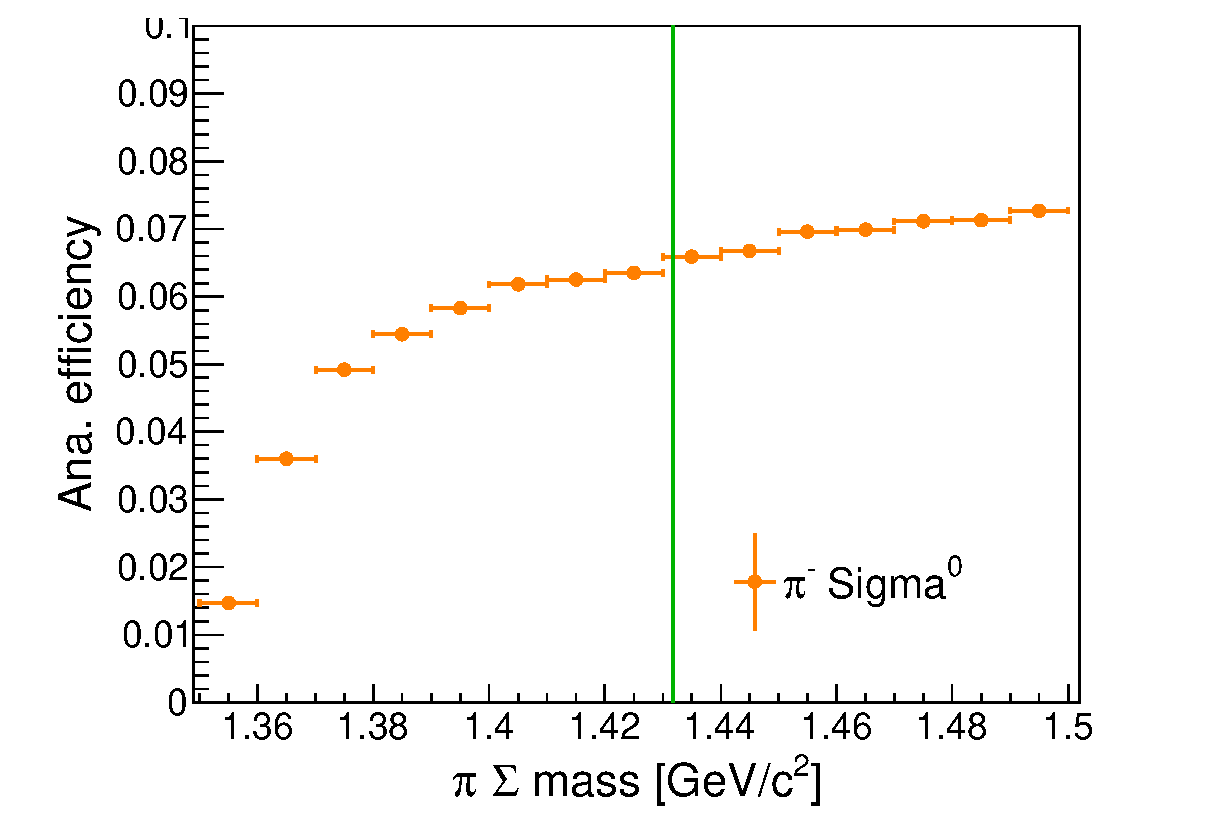
\includegraphics[width=8cm]{../pic/Dron/KP_ana/kp_acc.eps}
  \caption{
    This figure shows $d(K^-, p)"\pi^-\Sigma^0"$ acceptance
  }
  \label{fig:kp_acc}
\end{figure}


In the CDS acceptance correction,
the trigger event is defined on the condition that a forward-irradiated neutron or proton passes through the corresponding forward detector
and can be analyzed.
For example, in the case of forward neutrons,
the trigger event is defined by an event in which a forward-irradiated neutron passes through the NC
and produces an energy deposit above 8 MeVee in the NC.
An acceptable event is defined as
one where the same analysis procedure is applied to the real data and the event remains until the final selection.
For example, in the case of $d(K^-, n)\pi^{\mp} \Sigma^{\pm}$,
an acceptable event is one where $\pi^+$ and $\pi^-$ are detected individually in the CDS,
and the missing neutron can be identified from the $d(K^-, n \pi^+ \pi^-)$ missing mass,
while background contributions from $K^0$ and $\Sigma^{pm}_{forward}$ are removed.
In the case of $d(K^-, p)\pi^- \Sigma^0$, an acceptable event is one in which two $\pi^-$ are detected in the CDS,
$\Sigma^0$ is identified from the missing mass of $d(K^-, p \pi^-)$,
and the $p \gamma$ is determined from the missing mass of $d(K^-, p \pi^- \pi^-)$.
The CDS acceptances for $d(K^-, n)\pi^{\mp}\Sigma^{\pm}$ and $d(K^-, p)\pi^-\Sigma^0$,
obtained using these methods, are shown in Figures \ref{fig:kn_acc} and \ref{fig:kp_acc}, respectively.
By applying the CDS acceptance correction,
the double differential cross sections for $d(K^-, n)\pi^{\mp} \Sigma^{\pm}$ and $d(K^-, p)\pi^-\Sigma^0$ are obtained,
as shown in Figures \ref{fig:Charge_CS} and \ref{fig:pimS0_CS}.
The thin boxes indicate statistical errors, the thick boxes include fitting errors,
and the error bars represent the total errors, including those from conversion coefficients.

\begin{figure}[htbp]
  \centering
  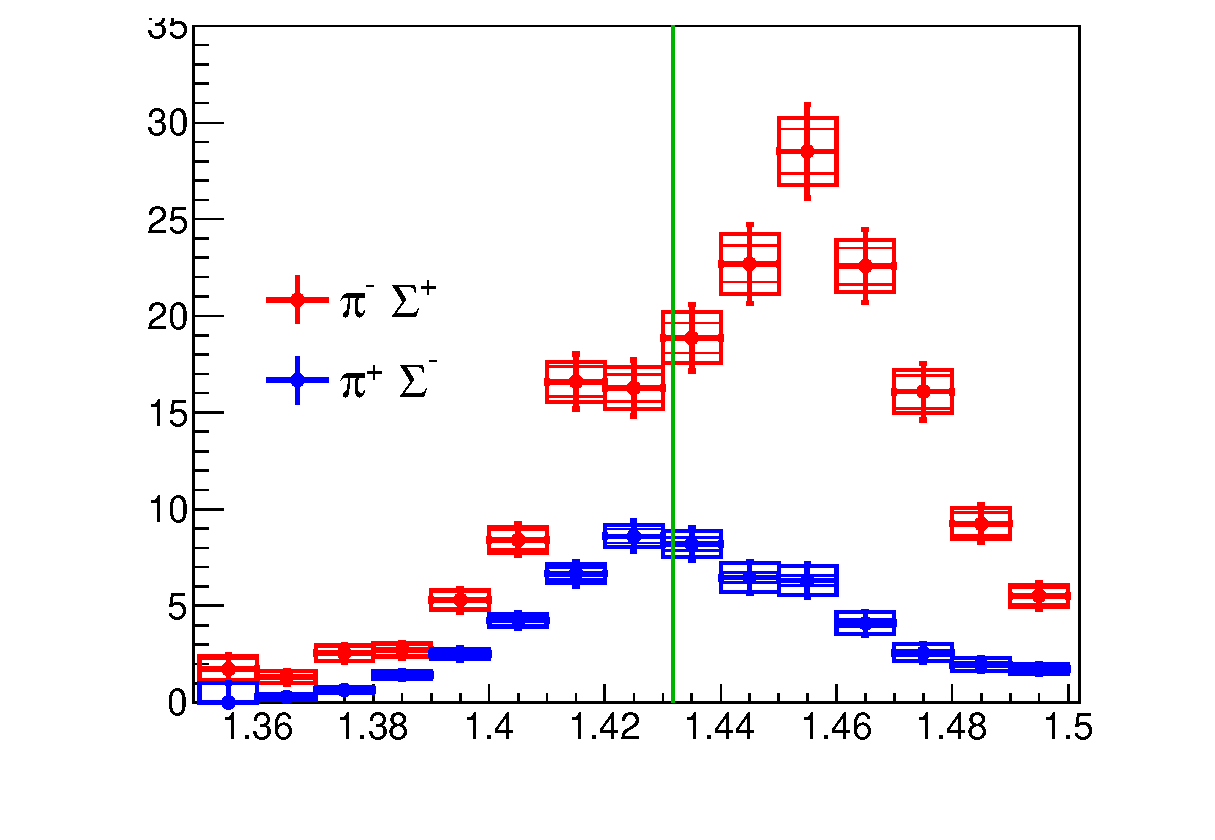
\includegraphics[width=9cm]{../pic/Dron/KN_ana/ChargeCS.eps}
  \caption{
    The red figure and blue figure shows about $d(K^-, n)"\pi^+\Sigma^-"$ and $d(K^-, n)"\pi^-\Sigma^+"$, respectively.
    The inner frame (thin line), outer frame (thick line), and error bars represent the addition of statistical errors, fitting errors, and conversion errors, which were calculated by root-mean-square.
    The green vertical lines indicates $\bar{K}N$ threshold.
  }
  \label{fig:Charge_CS}
\end{figure}

\begin{figure}[htbp]
  \centering
  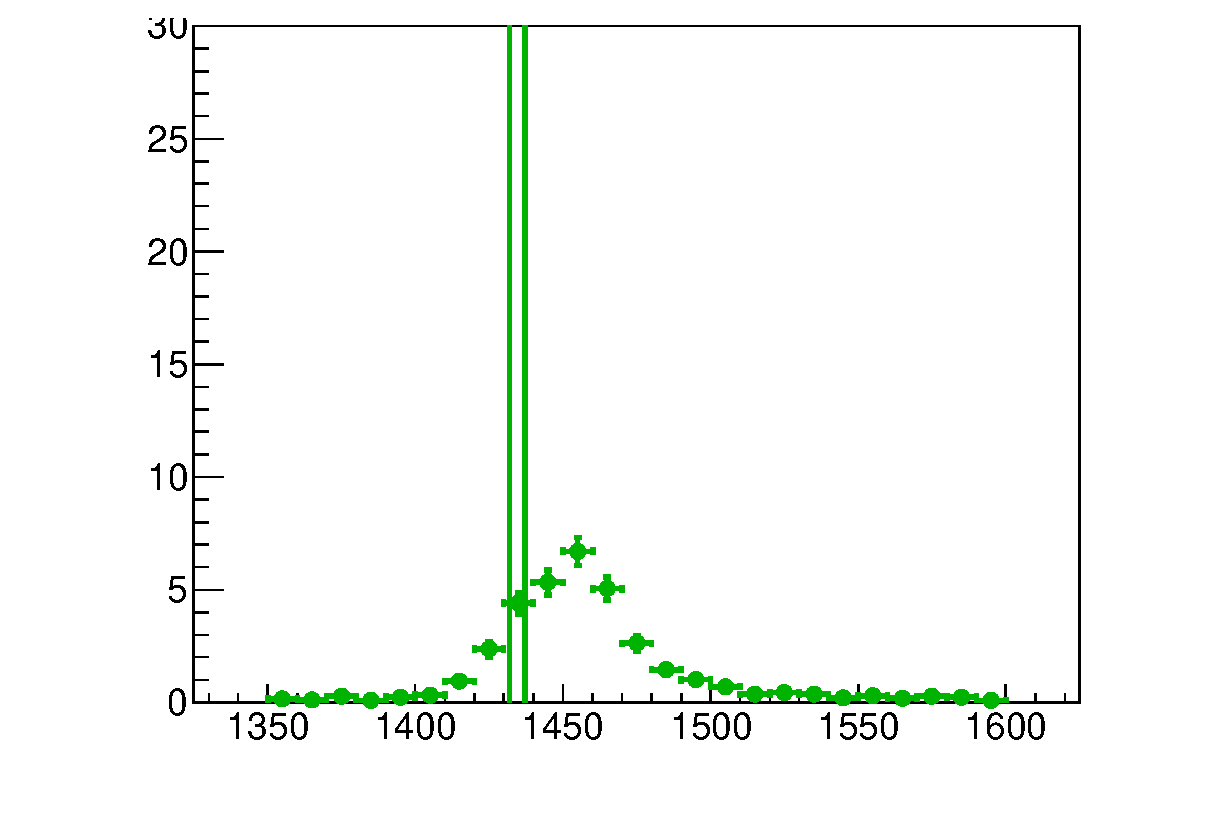
\includegraphics[width=9cm]{../pic/Dron/KP_ana/pimS0_CS.eps}
  \caption{
    This figure shows the cross section of $d(K^-, p)"\pi^- \Sigma^0"$.
    The box represents the statistical error, and the error bar represents the root mean squares of the conversion factor added to it.
    The green vertical lines indicates $\bar{K}N$ threshold.
  }
  \label{fig:pimS0_CS}
\end{figure}

